\documentclass[../../main/main.tex]{subfiles}
\graphicspath{{./figures/}}

\dominitoc
\faketableofcontents

\makeatletter
\renewcommand{\@chapapp}{M\'ecanique -- chapitre}
\makeatother

\toggletrue{student}
% \HideSolutionstrue
\toggletrue{corrige}
% \renewcommand{\mycol}{black}
\renewcommand{\mycol}{gray}

\begin{document}
\setcounter{chapter}{1}
\chapter{Dynamique du point}

\vfill

\begin{prgm}
	\begin{tcb}*(ror)"know"{Savoirs}
		\begin{itemize}
			\item Exploiter la conservation de la masse pour un système fermé.
			\item Établir l’expression de la quantité de mouvement pour un système de
			      deux points sous la forme~: $\pf=m\vf(\Gr)$.
			\item Première loi de \textsc{Newton}~: décrire le mouvement relatif de
			      deux référentiels galiléens.
			\item Force de gravitation. Modèle du champ de pesanteur uniforme au
			      voisinage de la surface d’une planète. Mouvement dans le champ de
			      pesanteur uniforme.
			\item Modèles d’une force de frottement fluide. Influence de la résistance
			      de l’air sur un mouvement de chute.
		\end{itemize}
	\end{tcb}
	\begin{tcb}*(ror)"how"{Savoir-faire}
		\begin{itemize}
			\item Troisième loi de \textsc{Newton}~: établir un bilan des forces sur un
			      système ou sur plusieurs systèmes en interaction et en rendre compte
			      sur un schéma.
			\item Deuxième loi de \textsc{Newton}~: déterminer les équations du
			      mouvement d’un point matériel ou du centre de masse d’un système fermé
			      dans un référentiel galiléen.
			\item Étudier le mouvement d’un système modélisé par un point matériel
			      dans un champ de pesanteur uniforme en l’absence de frottement.
			\item Exploiter, sans la résoudre analytiquement, une équation
			      différentielle~: analyse en ordres de grandeur, détermination de la
			      vitesse limite, utilisation des résultats obtenus par simulation
			      numérique. Écrire une équation adimensionnée.
		\end{itemize}
	\end{tcb}
\end{prgm}

\vfill

\newpage

\vspace*{\fill}
% \vfill
\minitoc
% \vfill
\vspace*{\fill}

\newpage

\section{Introduction}
Dans ce chapitre nous nous intéressons à étudier les causes de la mise en
mouvement d'un corps, représenté par un point matériel, et les mouvements qui en
découlent.

\subsection{Inertie et quantité de mouvement}
Mettre en mouvement un corps revient à en modifier la vitesse. Il est cependant
plus facile de mettre en mouvement (ou arrêter le mouvement) certains corps par
rapport à d'autres. Ce phénomène s'appelle l'inertie, et est
proportionnel à la masse d'un corps.

\begin{tcb*}(defi){Inertie et quantité de mouvement}
	La résistance d'un corps matériel de masse $m$ à varier de vitesse est
	appelée \textbf{inertie}, quantifié par la \textbf{masse} et le
	\textbf{vecteur quantité de mouvement} du point matériel M du corps~:
	\psw{
		\[
			\boxed{\pf\Rg(\Mr) = m\vf\Rg(\Mr)}
		\]
	}
	avec $\vf\Rg(\Mr)$ le vecteur vitesse du point M dans le référentiel $\Rc$.
\end{tcb*}

Il est en effet plus difficile de déplacer une voiture à l'arrêt qu'un caddie à
l'arrêt, et inversement il est plus difficile d'arrêter une voiture qu'un
caddie. Dans l'analogie électromécanique, c'est l'inductance $L$ qui s'oppose à
la variation du courant quand $m$ s'oppose à la variation de la vitesse.

\subsection{Forces fondamentales}
Les causes du mouvement d'un corps sont appelées \textbf{forces}.
\begin{tcb*}[sidebyside](defi){Forces}
	Les \textbf{forces} caractérisent les actions mécaniques sur un point matériel
	M. Ce sont des \textbf{vecteurs} et elles sont \textbf{indépendantes du
		référentiel}.
	\tcblower
	L'unité d'une force est le Newton, noté N, tel que~:
	\psw{
		\[\boxed{\SI{1}{N} = \SI{1}{kg.m.s^{-2}}}\]
	}
\end{tcb*}
Il existe quatre de ces forces que l'on caractérise de «~fondamentales~», qui
permettent de classer les interactions physiques entre les systèmes~:
% \begin{table}[htbp!]
% 	\centering
% 	\caption{Interactions fondamentales}
% 	\begin{tabularx}{\linewidth}{YYYYY}
% 		\toprule
% 		\textbf{Interaction}                         &
% 		\textbf{Intensité}                           &
% 		\textbf{Portée}                              &
% 		\textbf{Sujet}                               &
% 		\textbf{Conséquences}
% 		\\
% 		\midrule
% 		Faible                                       &
% 		Faible                                       &
% 		Extrême\mnt\ courte ($\approx \SI{e-18}{m}$) &
% 		Fermions                                     &
% 		Désintégration radioactive, fusion nucléaire
% 		\\
% 		\addlinespace[0.5em]
% 		Forte                                        &
% 		Très forte                                   &
% 		Très courte ($\approx \SI{e-14}{m}$)         &
% 		Quarks et gluons                             &
% 		Cohésion des nucléons
% 		\\
% 		\addlinespace[0.5em]
% 		Électromagnétique                            &
% 		Forte                                        &
% 		Longue                                       &
% 		Particules chargées                          &
% 		Cohésion des matériaux, propriétés mécaniques
% 		\\
% 		\addlinespace[0.5em]
% 		Grativationnelle                             &
% 		Faible                                       &
% 		Très longue                                  &
% 		Particules massives                          &
% 		Poids, organisation cosmique
% 		\\
% 		\bottomrule
% 	\end{tabularx}
% 	\label{tab:int_fond}
% \end{table}

\begin{table}[htbp!]
	\centering
	\caption{Interactions fondamentales}
	\begin{tabularx}{\linewidth}{lYYYY}
		\toprule
		\diagbox{\textbf{Caract.}}{\textbf{Type}}           &
		\psw{\textbf{Faible}}                               &
		\psw{\textbf{Forte}}                                &
		\psw{\textbf{Électromag.}}                          &
		\psw{\textbf{Grativationnelle}}
		\\
		\midrule
		Intensité                                           &
		\psw{Faible}                                        &
		\psw{Très forte}                                    &
		\psw{Forte}                                         &
		\psw{Faible}
		\\
		\addlinespace[0.5em]
		Portée                                              &
		\psw{Extrême\mnt\ courte ($\approx \SI{e-18}{m}$)}  &
		\psw{Très courte ($\approx \SI{e-14}{m}$)}          &
		\psw{Longue}                                        &
		\psw{Très longue}
		\\
		\addlinespace[0.5em]
		Sujet                                               &
		\psw{Fermions}                                      &
		\psw{Quarks et gluons}                              &
		\psw{Particules chargées}                           &
		\psw{Particules massives}
		\\
		\addlinespace[0.5em]
		Conséquences                                        &
		\psw{Désintégration radioactive, fusion nucléaire}  &
		\psw{Cohésion des nucléons}                         &
		\psw{Cohésion des matériaux, propriétés mécaniques} &
		\psw{Poids, organisation cosmique}
		\\
		\bottomrule
	\end{tabularx}
	\label{tab:int_fond}
\end{table}
% \begin{itemize}
% 	\item \textbf{L'interaction faible}~: elle intervient au niveau des
% 	      \textbf{nucléons}, est de \textit{faible intensité} et de
% 	      \underline{très courte portée} ($\approx \SI{e-18}{m}$)~;
% 	\item \textbf{L'interaction forte}~: responsable de la cohésion des
% 	      \textbf{noyaux atomiques}, et permet aux protons de rester dans
% 	      le noyau
% 	      malgré la répulsion électromagnétique due à leurs charges électriques
% 	      identiques. Elle est de \textit{très forte intensité} mais sur une
% 	      \underline{très courte portée} ($\approx \SI{e-14}{m}$).
% 	\item \textbf{L'interaction électromagnétique}~: elle intervient entre les
% 	      \textbf{particules chargées}, avec une \textit{forte intensité} et à
% 	      \underline{longue portée}. Les particules de même signe se repoussent,
% 	      tandis que celles de signes opposées s'attirent, et est responsable de
% 	      la \textbf{cohésion des matériaux} et de leurs propriétés mécaniques
% 	      (dureté, viscosité, propriétés chimiques…).
% \end{itemize}

\begin{tcb*}(prop){Interaction électrostatique}
	Avec l'interaction électrostatique, les particules de même signe se repoussent,
	tandis que celles de signes opposées s'attirent. Elle est responsable de
	la \textbf{cohésion des matériaux} et de leurs propriétés mécaniques
	(dureté, viscosité, propriétés chimiques…).
	\smallbreak
	La force d'interaction électrostatique subie par une particule de charge
	$q_A$ de la part d'une charge $q_B$ est~:
	\smallbreak
	\begin{isd}
		\psw{
			\[
				\Ff_{e,\rm B\ra A} = \frac{1}{4\pi\ep_0} \frac{q_Aq_B}{\rm BA^2}\ur
				\qavec
				\ur = \frac{\vv{\rm BA}}{\rm BA}
			\]
		}
		$\ur$ est un vecteur unitaire dirigé de B vers A.
		\tcblower
		\begin{center}
			\sswitch{
				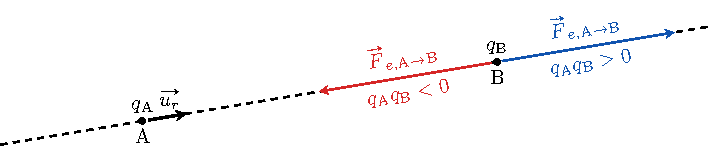
\includegraphics[width=\linewidth, draft=true]{fe}
			}{
				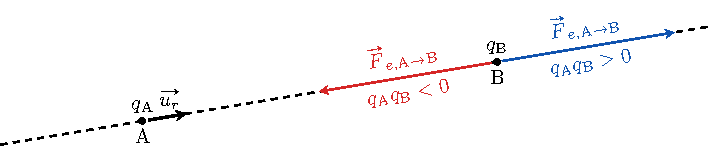
\includegraphics[width=\linewidth]{fe}
			}
			\vspace{-15pt}
			\captionof{figure}{Interaction électrostatique.}
		\end{center}
	\end{isd}
\end{tcb*}

% \begin{itemize}
% 	\item \textbf{L'interaction gravitationnelle}~: elle intervient entre les
% 	      \textbf{particules massives} et est à \textit{faible intensité} mais à
% 	      \ul{très longue portée}. La masse étant une grandeur positive, toutes
% 	      les massives s'attirent entre elles. Elle prédomine à l'échelle
% 	      astronomique et à l'origine du poids, et indirectement de la poussée
% 	      d'\textsc{Archimède}.
% \end{itemize}
\begin{tcb*}(prop){Interaction gravitationnelle}
	Avec l'interaction gravitationnelle, la masse étant une grandeur positive,
	toutes les massives s'attirent entre elles. Elle prédomine à l'échelle
	astronomique.
	\smallbreak
	La force d'interaction gravitationnelle subie par une masse
	$m_A$ de la part d'une masse $m_B$ est~:
	\smallbreak
	\begin{isd}
		\psw{
			\[
				\Ff_{g,\rm B\ra A} = -\Gc \frac{m_Am_B}{\rm BA^2}\ur
				\qavec
				\ur = \frac{\vv{\rm BA}}{\rm BA}
			\]
		}
		$\ur$ est un vecteur unitaire dirigé de B vers A.
		\tcblower
		\begin{center}
			\sswitch{
				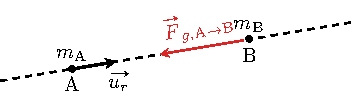
\includegraphics[width=\linewidth, draft=true]{fg}
			}{
				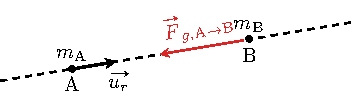
\includegraphics[width=\linewidth]{fg}
			}
			\vspace{-15pt}
			\captionof{figure}{Interaction gravitationnelle.}
		\end{center}
	\end{isd}
\end{tcb*}

\section{Les trois lois de \textsc{Newton} (1687)}
\subsection{Principe d'inertie}

\begin{tcb*}(prop){Première loi de \textsc{Newton}~: principe d'inertie}
	Il existe des référentiels appelés \textbf{référentiels galiléens} dans
	lesquels un point matériel M soumis à \textbf{aucune action mécanique} est
	\begin{itemize}
		\item \psw{soit \textbf{au repos}~;}
		\item \psw{soit en \textbf{translation rectiligne uniforme}.}
	\end{itemize}
	Ainsi, tout référentiel en translation rectiligne uniforme par rapport à un
	référentiel galiléen est galiléen.
\end{tcb*}

Ils n'existent rigoureusement aucun référentiel galiléen, mais on peut en
considérer certains comme \textit{approximativement} galiléens lorsqu'on étudie
le problème sur \textbf{une durée assez courte}. En reprenant les exemples du
chapitre précédent~:
\begin{itemize}
	\item Le référentiel \textbf{héliocentrique} est supposé galiléen si le
	      mouvement étudié est plus court qu'un trajet significatif du Soleil dans
	      la galaxie, soit plusieurs \textbf{millions d'années}~;
	\item Le référentiel \textbf{géocentrique} est supposé galiléen si le
	      mouvement étudié est plus court qu'un trajet significatif de la Terre
	      autour du Soleil, soit \textbf{une année}~;
	\item Les référentiels \textbf{terrestres} sont supposés galiléens si le
	      mouvement étudié est plus court qu'une rotation significative de la
	      Terre, soit \textbf{une journée}.
\end{itemize}

\subsection{Principe fondamental de la dynamique}

C'est une des lois les plus importantes de la physique, permettant de relier le
mouvement cinématique (dérivée de la vitesse) d'un corps en fonction de ses
causes (les forces extérieures).

\begin{tcb*}(prop){Deuxième loi de \textsc{Newton}~: principe fondamental de la
			dynamique}

	Dans un référentiel galiléen $\Rc$, la dérivée temporelle du vecteur
	quantité de mouvement $\pf\Rg(\Mr)$ d'un point matériel M de masse $m$ est
	égale à la somme des forces extérieures agissant sur le système
	$\Ff_{\ext\ra\Mr}$~:
	\psw{
		\[
			\boxed{\dv{\pf\Rg(\Mr)}{t} = \sum \Ff_{\ext\ra\Mr}}
		\]
	}
	Lorsque le \textbf{système est fermé} et donc la \textbf{masse est constante},
	on a $\forall t$ $\pf\Rg(\Mr) = m\vf\Rg(\Mr)$, ainsi
	\psw{
		\[
			\boxed{m\af\Rg(\Mr) = \sum \Ff_{\ext\ra\Mr}}
		\]
	}
	avec $\af\Rg(\Mr)$ le vecteur accélération du point M.
\end{tcb*}

\begin{tcb*}(rema)<lfnt>'l'{Remarque}
	Certains mouvements ne peuvent donc pas être traités avec cette dernière
	formulation s'ils s'accompagnent d'une variation de masse~:
	\begin{itemize}
		\item \psw{Le mouvement d'une fusée qui brûle son carburant puis abandonne
			      ses réservoirs~;}
		\item \psw{Le mouvement d'une goutte d'eau qui s'évapore lors de sa chute.}
	\end{itemize}
	Dans ces cas-là, on utilise la première formulation.
\end{tcb*}

\subsection{Loi des actions réciproques}

\begin{tcb*}[sidebyside](prop){Troisième loi de \textsc{Newton}~:%
			loi des actions réciproques}
	Pour deux points M$_1$ et M$_2$ en interaction, la force exercée par le point
	1 sur le point 2 est égale à l'\textbf{opposé} de la force exercée par le
	point 2 sur le point 1~:
	\psw{
		\[\boxed{\Ff_{1\ra2} = - \Ff_{2\ra1}}\]
	}
	\tcblower
	\begin{minipage}{0.45\linewidth}
		\begin{center}
			\sswitch{
				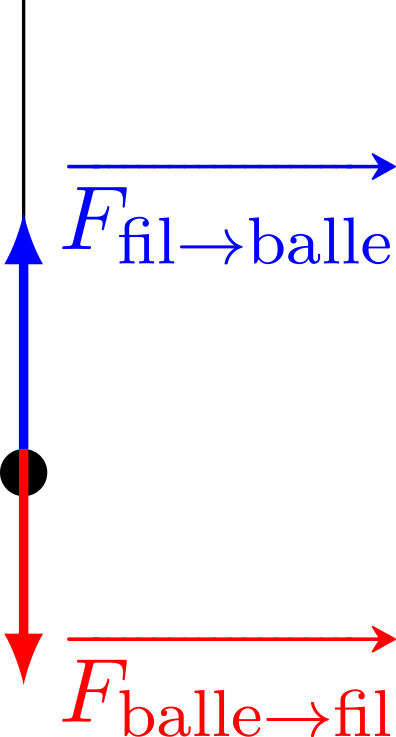
\includegraphics[height=2.6cm, draft=true]{loi3a}
			}{
				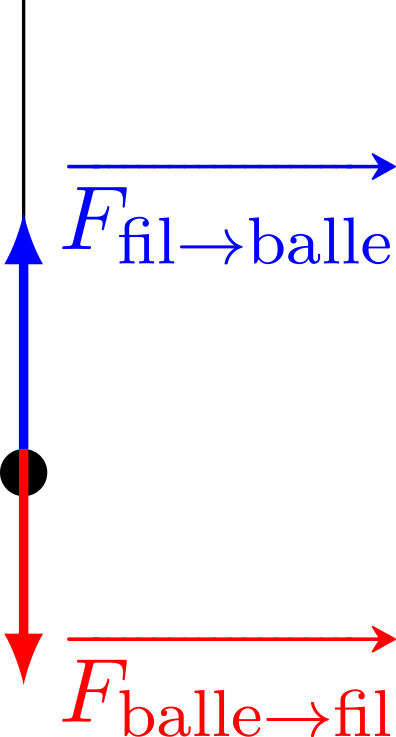
\includegraphics[height=2.6cm]{loi3a}
			}
			\captionof{figure}{Balle avec fil.}
		\end{center}
	\end{minipage}
	\hfill
	\begin{minipage}{0.45\linewidth}
		\begin{center}
			\sswitch{
				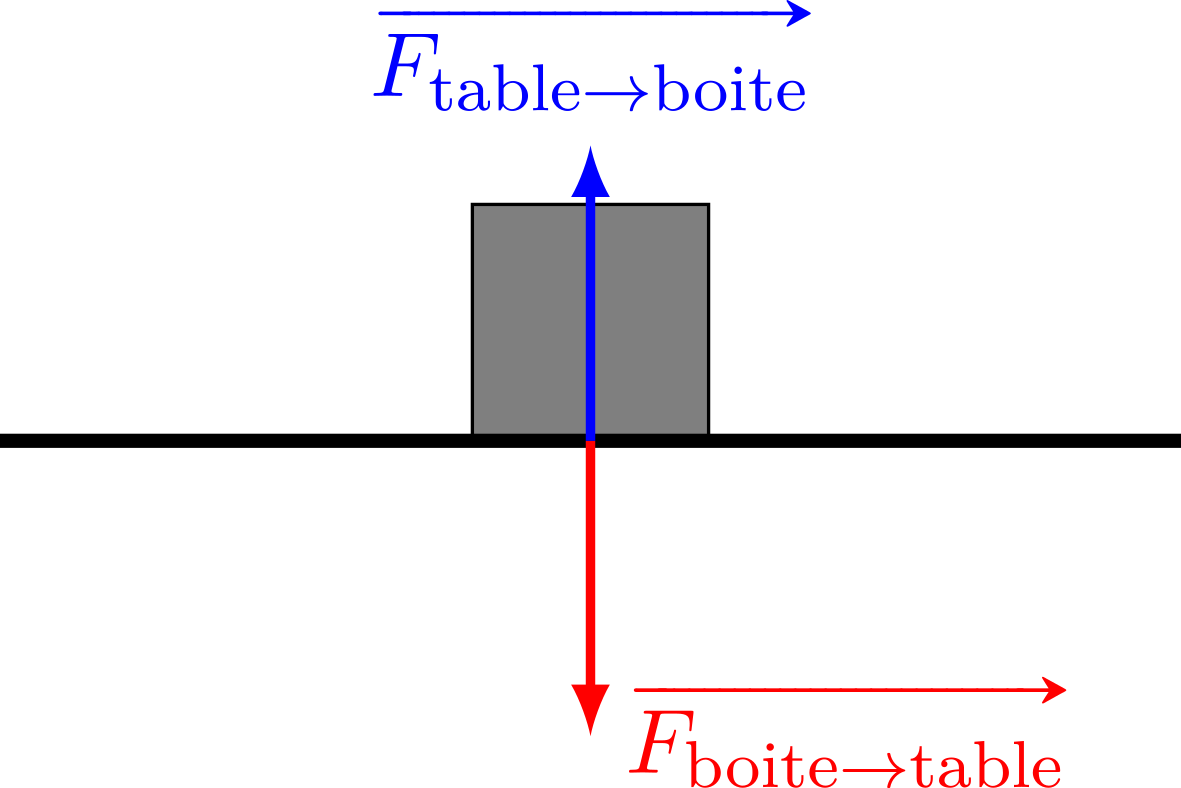
\includegraphics[height=2.6cm, draft=true]{loi3b}
			}{
				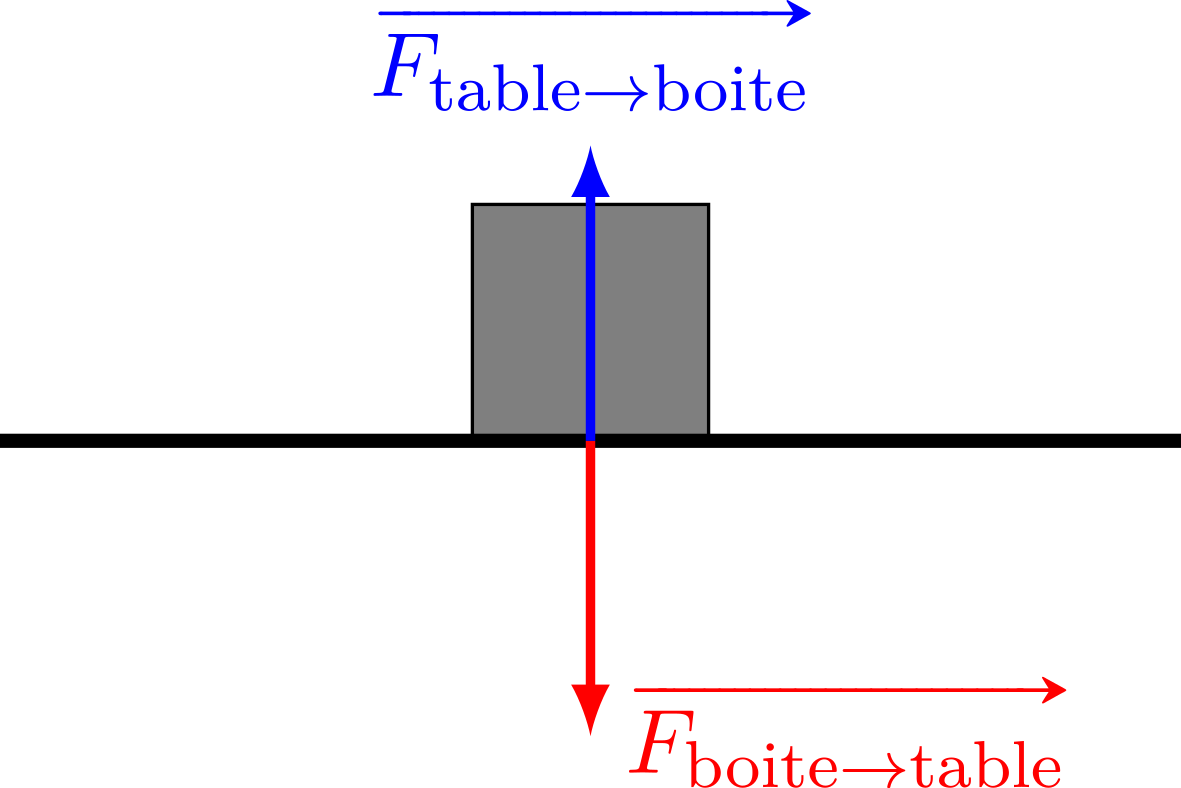
\includegraphics[height=2.6cm]{loi3b}
			}
			\vspace{-15pt}
			\captionof{figure}{Boîte sur table.}
		\end{center}
	\end{minipage}
\end{tcb*}

\section{Ensembles de points}
Aucun système n'est rigoureusement ponctuel, mais sous certaines conditions il
est possible d'étudier le mouvement d'un corps en tant que point matériel de
manière rigoureuse. Établissons ce comportement.

\subsection{Centre d'inertie}

\begin{tcb*}(defi){Centre d'inertie}
	Le \textbf{centre d'inertie} ou \textbf{centre de gravité} G d'un ensemble
	de points matériels M$_i$ de masses $m_i$ est défini par~:
	\[
		\psw{
			\boxed{\vv{\rm OG} = \sum_i \frac{m_i}{m_{\tot}} \vv{{\OMr}_i}}
		}
		\Lra
		\psw{
			\boxed{\sum_i m_i \vv{\rm GM_i} = \of }
		}
	\]
	Il s'agit du barycentre des points du système, pondéré par leur masse.
\end{tcb*}

Le centre d'inertie correspond au \textbf{centre d'équilibre gravitationnel}
d'un ensemble de point. Ainsi, pour mettre une règle en équilibre
horizontalement il faut la reposer en son milieu. Un marteau, en revanche, a son
centre d'inertie bien plus proche de la masse que du milieu.

On peut démontrer l'équivalence entre les deux définitions~:
\begin{tcb*}(demo){Centre d'inertie}
	\psw{
		\begin{gather*}
			m_{\tot} = \sum_i m_i \Ra
			\sum_i m_i\vv{\rm OG} = \sum_i m_i\vv{\OMr_i}
			\Lra
			\of                   = \sum_i m_i \left( \vv{\OMr_i} - \vv{\rm OG} \right)
		\end{gather*}
		Or, comme $\vv{\OMr_i} - \vv{\rm OG} = \vv{\rm GO} + \vv{\OMr_i} = \vv{\rm
				GM_i}$, on aura bien~:
		\[
			\boxed{\sum_i m_i\vv{{\rm GM}_i} = \of}
		\]
	}
\end{tcb*}

\begin{tcb*}[breakable](appl)<lfnt>'l'{Application}
	Soient 2 masses placées en A et en B. Déterminer la position de G en
	calculant $\vv{\rm AG}$ dans les deux cas suivants~:
	\begin{tasks}(2)
		\task[\fbox{1}]
		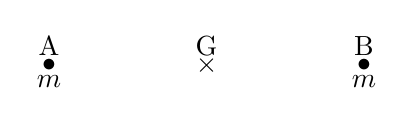
\begin{tikzpicture}[]
			\coordinate (A) at (-2,0);
			\coordinate (B) at (2,0);
			\coordinate (G) at (0,0);
			\node[] at (A) {$\bullet$};
			\node[below] at (A) {$m$};
			\node[above] at (A) {A};
			\node[] at (B) {$\bullet$};
			\node[below] at (B) {$m$};
			\node[above] at (B) {B};
			\node[] at (G) {$\times$};
			\node[above] at (G) {G};
		\end{tikzpicture}
		\task[\fbox{2}]
		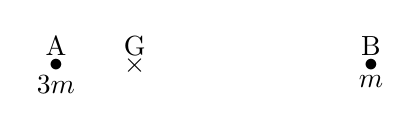
\begin{tikzpicture}[]
			\coordinate (A) at (-2,0);
			\coordinate (B) at (2,0);
			\coordinate (G) at (-1,0);
			\node[] at (A) {$\bullet$};
			\node[below] at (A) {$3m$};
			\node[above] at (A) {A};
			\node[] at (B) {$\bullet$};
			\node[below] at (B) {$m$};
			\node[above] at (B) {B};
			\node[] at (G) {$\times$};
			\node[above] at (G) {G};
		\end{tikzpicture}
	\end{tasks}
	\tcblower
	\begin{enumerate}
		\mitem \psw{
			\begin{gather*}
				m\vv{\rm GA} + m\vv{\rm GB} = \of
				\Lra \vv{\rm GA} + \vv{\rm GB} = \of
				\intertext{
					Or,
					$\vv{\rm GA} + \vv{\rm GB} =
						\vv{\rm GA} + \vv{\rm GA} + \vv{\rm AB}$,
					donc
				}
				2\vv{\rm GA} + \vv{\rm AB} = \of
				\Lra
				2\vv{\rm AG}               = \vv{\AB}
				\Lra
				\boxed{\vv{\rm AG}        = \frac{1}{2}\vv{\rm AB}}
			\end{gather*}
		}
		\mitem \psw{
			\begin{gather*}
				3m\vv{\rm GA} + m\vv{\rm GB} = \of
				\Lra 3\vv{\rm GA} + \vv{\rm GB} = \of
				\intertext{
					Or,
					$3\vv{\rm GA} + \vv{\rm GB} =
						3\vv{\rm GA} + \vv{\rm GA} + \vv{\rm AB}$,
					donc
				}
				4\vv{\rm GA} + \vv{\AB} = \of
				\Lra
				4\vv{\rm AG}            = \vv{\AB}
				\Lra
				\boxed{\vv{\rm AG}     = \frac{1}{4}\vv{\rm AB}}
			\end{gather*}
		}
		\vspace{-15pt}
	\end{enumerate}
\end{tcb*}

Cette définition peut être étendue aux solides qui peuvent être vus comme un
ensemble infini de points infiniment proches. Dans ce cas, la somme discrète
devient une intégrale.

\subsection{Quantité de mouvement d'un ensemble de points}

On souhaiterait pouvoir étudier un ensemble de points comme le mouvement d'un
point unique, comme le centre d'inertie. Pour cela, il faut étudier la quantité
de mouvement d'un ensemble de points.

\begin{tcb*}(defi){Quantité de mouvement d'un ensemble de points}
	Le vecteur quantité de mouvement d'un ensemble $\Sc$ de points matériels
	M$_i$ de masses $m_i$ est la somme des quantités de mouvement de chacun des
	points~:
	\psw{
		\[
			\boxed{\pf(\Sc) = \sum_i m_i \vf(\Mr_i)}
		\]
	}
\end{tcb*}

\begin{tcb*}[cnt, bld](prop){Quantité de mouvement et centre d'inertie}
	La quantité de mouvement d'un ensemble de points est la quantité de
	mouvement d'un point matériel placé en $G$ et de masse $m_{\tot}$~:
	\psw{
		\[
			\boxed{\pf (\Sc) = m_{\tot}\vf (\Gr)}
		\]
	}
	Tout se passe comme si la masse était concentrée en G.
\end{tcb*}

\begin{tcb}(demo){Quantité de mouvement et centre d'inertie}
	Pour que les choses soient simples, il faudrait donc que $\pf(\Sc)$ soit relié
	au centre d'inertie. Or,
	\psw{
		\[
			\vf(\Gr) = \dv{\vv{\rm OG}}{t} = \frac{1}{m_{\tot}}
			\underbracket[1pt]{\sum_i m_i \dv{{\OM}_i}{t}}_{\pf(\Sc)}
			\Lra
			\boxed{\pf(\Sc) = m_{\tot}\vf(\Gr)}
		\]
	}
\end{tcb}

\subsection{Théorème de la résultante cinétique}
Si on peut étudier la cinématique d'un corps par l'étude de son centre de
gravité, comment les forces interviennent-elles sur cet ensemble de points~?
Considérons pour simplifier un système de deux points M$_1$ et M$_2$ de masses
$m_1$ et $m_2$ en mouvement dans un référentiel galiléen. On peut appliquer le
principe fondamental de la dynamique à chacun d'entre eux~:
\psw{
	\[\dv{\pf(\Mr_1)}{t} = \Ff_{\Mr_2\ra\Mr_1} + \Ff_{\ext\ra\Mr_1}\]
}
avec deux types de forces~: les forces intérieures du système, ici celles
exercées par M$_2$ sur M$_1$, et les forces extérieures, c'est-à-dire toutes les
autres. En faisant de même pour M$_2$~:
\psw{
	\[\dv{\pf(\Mr_2)}{t} = \Ff_{\Mr_1\ra\Mr_2} + \Ff_{\ext\ra\Mr_2}\]
}
Ainsi, avec la définition de la quantité de mouvement d'un ensemble de points,
\psw{
	\[
		\dv{\pf(\Sc)}{t} =
		\underbracket[1pt]{\Ff_{\Mr_1\ra\Mr_2}+\Ff_{\Mr_2\ra\Mr_1}}_{= \of
			\text{ d'après la 3ème loi}} + \Ff_{\ext\ra\Mr_1} + \Ff_{\ext\ra\Mr_2}\]
}

\begin{tcb*}(prop){Théorème de la résultante cinétique}
	Le principe fondamental de la dynamique pour un point matériel s'applique à un
	ensemble de point en prenant pour point matériel le centre d'inertie G affecté
	de la masse totale $m_{\tot}$ du système, en ne considérant que les
	\textbf{forces extérieures} s'appliquant à l'ensemble~: \psw{
		\[\boxed{m_{\tot}\dv{\vf(\Gr)}{t} = \sum \Ff_{\ext}}\]
	}
\end{tcb*}

\begin{tcb*}(ror){Conclusion}
	Le mouvement du centre de gravité n’est affecté que par les forces extérieures
	au système. Ainsi, dans la suite, on étudiera le \textbf{mouvement du centre
		de gravité}, de masse $m_{\tot}$, soumis aux \textbf{forces extérieures} au
	système.
\end{tcb*}

\subsection{Méthode générale de résolution en mécanique}
\begin{enumerate}[label=\sqenumi]
	\bitem{Système} Quel est l'objet en mouvement, dans quel
	référentiel étudie-t-on le mouvement~?

	\bitem{Schéma.} Faire un schéma du problème dans une \textbf{situation
		quelconque}\ftn{On ne fait \textbf{jamais} de schéma à l'équilibre ou à des
		angles particuliers (45\degree\ par exemple)}.

	\bitem{Modélisation.} Donner le repère, détailler le repérage, les conditions
	initiales, les représenter sur le schéma et \textit{définir les notations}
	nécessaires.

	\bitem{Bilan des forces.} Faire le bilan des forces, les exprimer \textbf{dans
		le repère} choisi et les représenter sur le schéma.

	\bitem{Deuxième loi de \textsc{Newton}.} Appliquer le PFD au système.

	\bitem{Équations scalaires.} Donner les trois équations $\ddot{x}$,
	$\ddot{y}$ et $\ddot{z}$.

	\bitem{Répondre aux questions.} Le plus souvent, obtenir les équations
	horaires $x(t)$, $y(t)$ et $z(t)$.
\end{enumerate}

% \begin{tcb}*(expe)<itc>"trans"{Transition}
% 	Avec ces outils, voyons maintenant quelques forces et situations usuelles
% 	que l'on rencontrera en dynamique.
% \end{tcb}

\section{Forces usuelles}
\subsection{Le poids}
\subsubsection{Définition}

\begin{tcb*}[sidebyside](defi){Poids et pesanteur}
	Dû à l'attraction gravitationnelle de la Terre, un corps de masse $m$ à sa
	surface subit une force que l'on appelle le \textbf{poids}, telle que~:
	\psw{
		\[\boxed{\Pf = m\gf = -mg\uz}\]
	}

	avec $\gf$ le vecteur \textbf{accélération de la pesanteur}, de norme $g =
		\norm{\gf} = \SI{9.81}{m.s^{-2}}$ et dirigé \textbf{verticalement vers le
		sol}.
	\tcblower
	Par définition de l'interaction gravitationnelle, on a
	\psw{
	\[\gf = -\Gc \frac{m_T}{R_T{}^2}\uz\]
	}
	avec $m_T$ et $R_T$ la masse et le rayon de la Terre, $\Gc$ la constante
	gravitationnelle, et $\uz$ vertical ascendant.
\end{tcb*}

\subsubsection{La chute libre}
\begin{tcb*}(defi)<lfnt>'l'{Chute libre}
	Un système en chute libre pure ne subit que l'action de son poids.
\end{tcb*}

\noindent
\begin{minipage}[t]{0.65\linewidth}
	\begin{enumerate}[label=\sqenumi]
		\bitem{Système.} \psw{
			\{balle\} dans $\Rc\ind{labo}$, supposé galiléen.
		}
		\bitem{Schéma}.
	\end{enumerate}
\end{minipage}
\hfill
\begin{minipage}[t]{0.30\linewidth}
	\begin{center}
		\vspace{-12pt}
		\sswitch{
			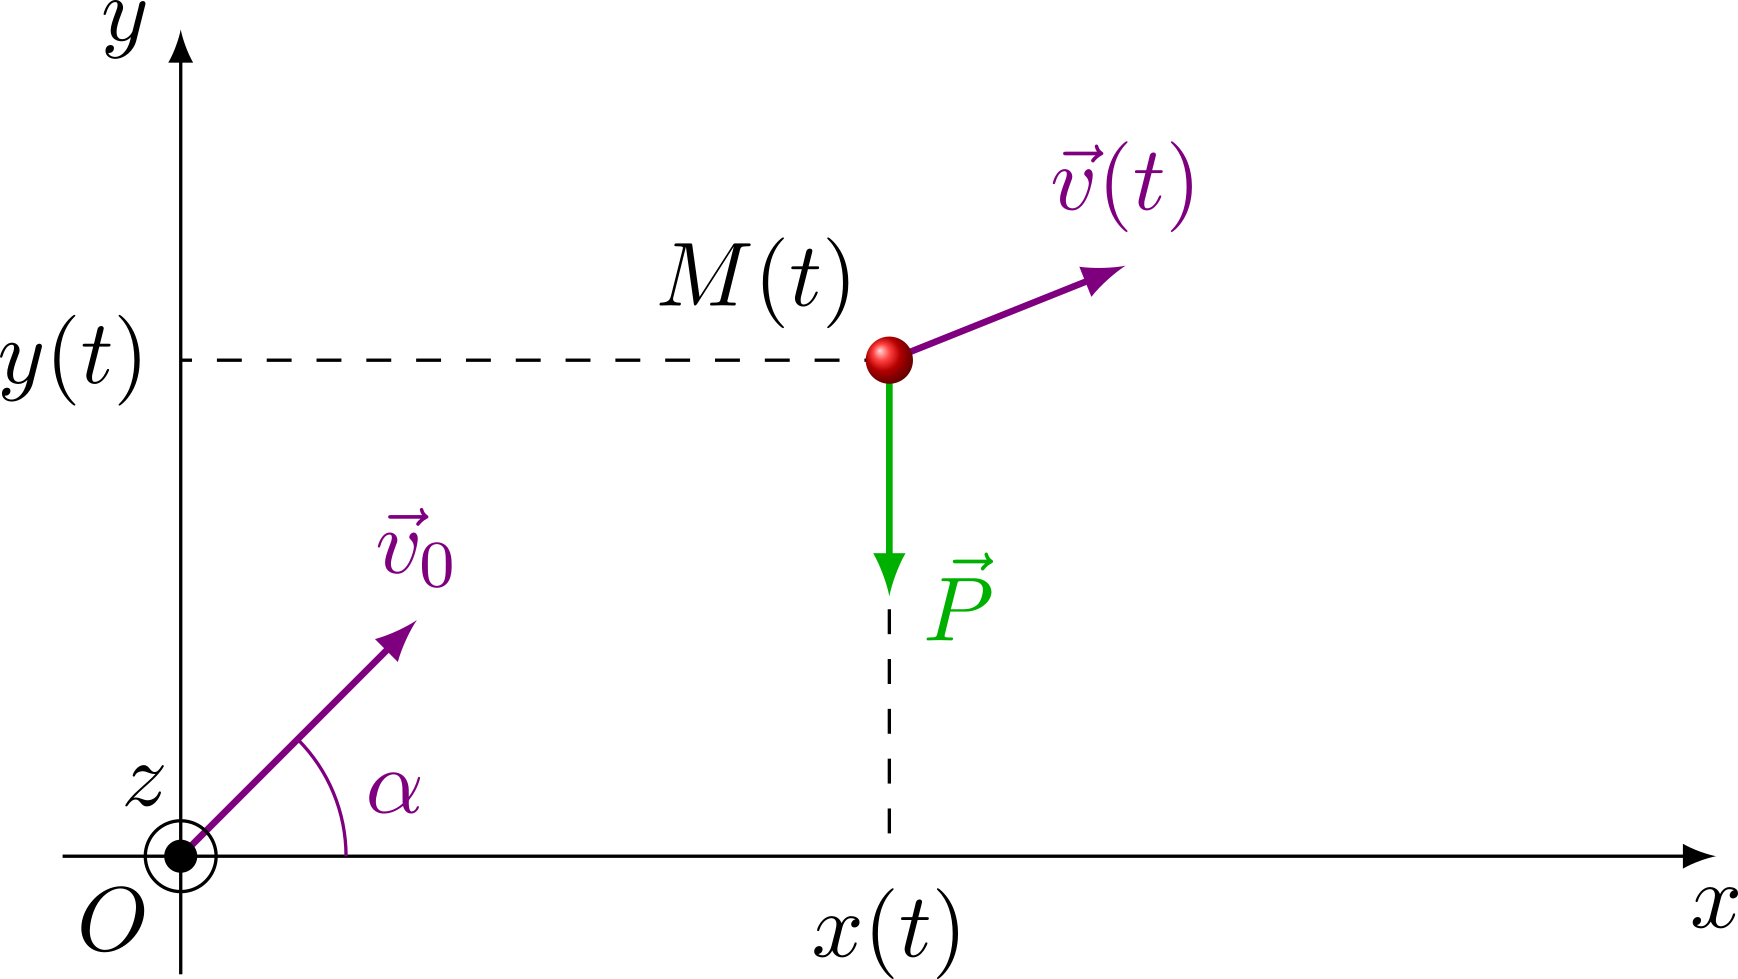
\includegraphics[width=\linewidth, draft=true]{cl_ssf}
		}{
			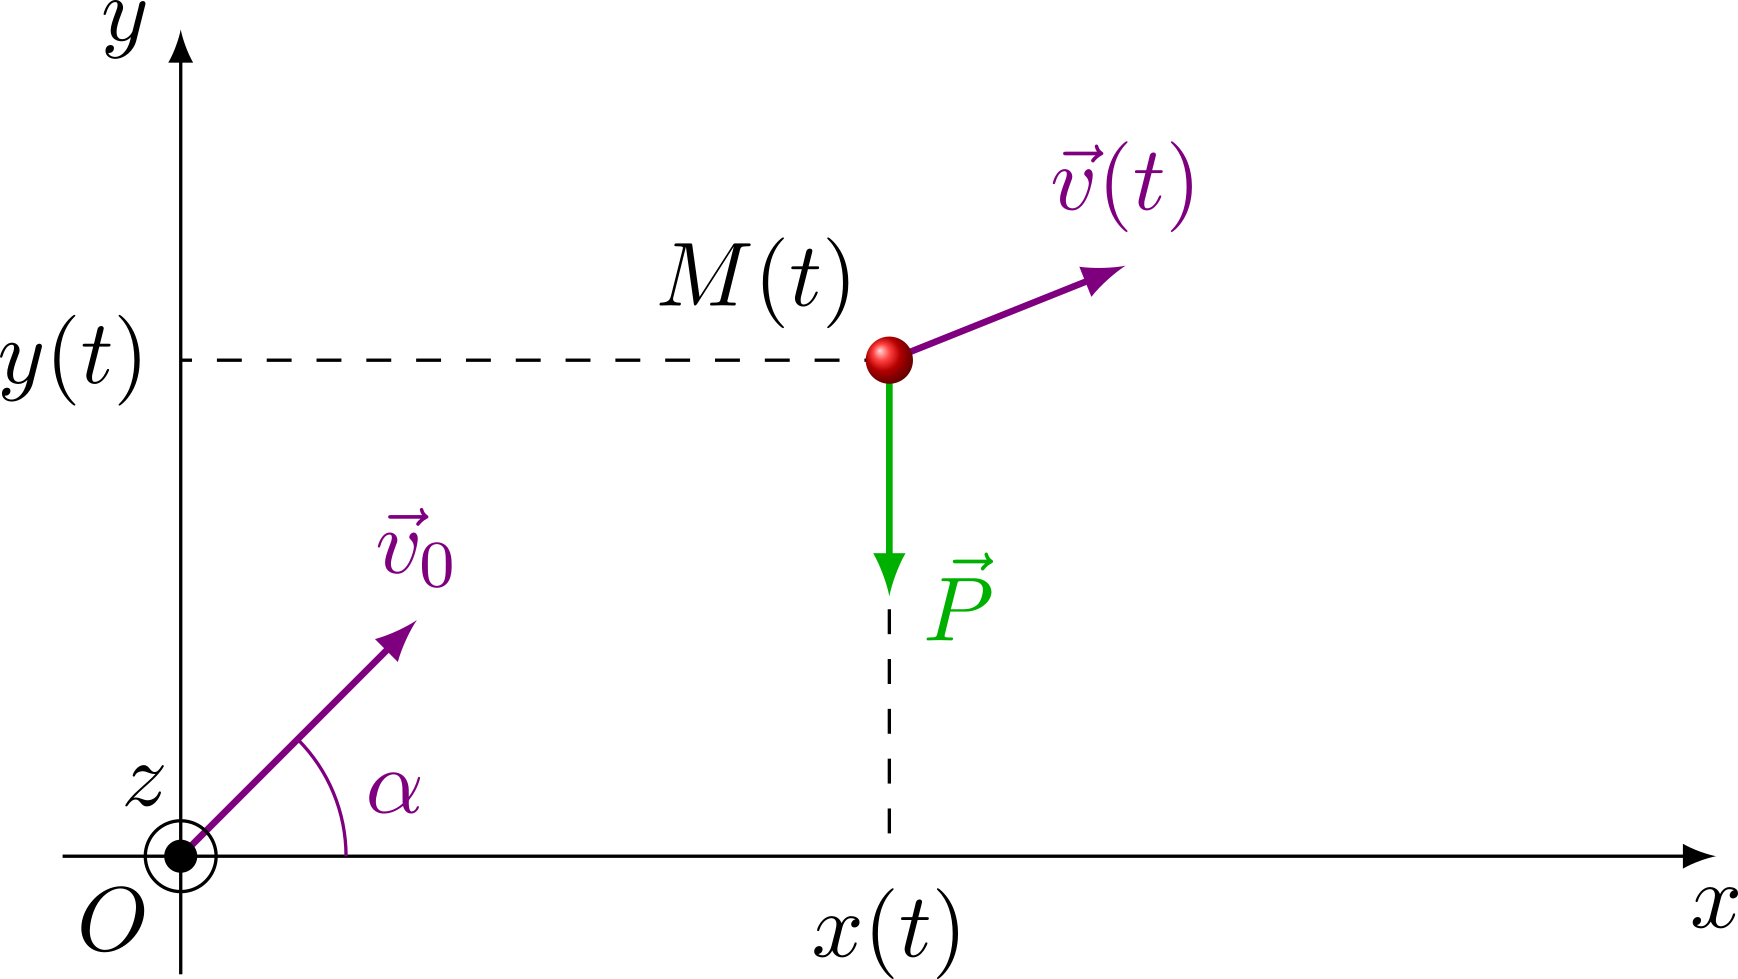
\includegraphics[width=\linewidth]{cl_ssf}
		}
		\vspace{-15pt}
		\captionof{figure}{Chute libre.}
	\end{center}
\end{minipage}
\begin{enumerate}[label=\sqenumi, start=3]
	\vspace{-40pt}
	\bitem{Modélisation}.
	\begin{itemize}
		\item Repère~: $(\ux, \uy, \uz)$ base orthonormée directe (BOND) avec $\ux$
		      dans le sens du lancer et $\uy$ verticale ascendante.
		\item Repérage~:
		      \psw{
			      \begin{align*}
				      \OM & = x\ux + y\uy       \\
				      \vf & = \xp\ux + \yp\uy   \\
				      \af & = \xpp\ux + \ypp\uy
			      \end{align*}
		      }
		      \vspace{-15pt}
		\item Conditions initales~:
		      \[
			      \psw{
				      \OM(0) = \of
			      }
			      \qet
			      \psw{
				      \vf(0) = v_0\cos\alpha\ux + v_0\sin\alpha\uy
			      }
		      \]
		      avec $\alpha$ l'angle du vecteur $\vfo$ avec l'axe
		      horizontal et $v_0$ sa norme.
	\end{itemize}
	\bitem{Bilan des forces.}
	\psw{
		Ici, seul le poids s'applique~:
		\[
			\begin{array}{ll}
				\textbf{Poids} & \Pf = m\gf = -mg\uy
			\end{array}
		\]
	}
	\item \leftcenters{\textbf{PFD.}}{\psw{$m\af = \Pf$}}
	      \bitem{Équations scalaires.} On projette sur les axes~:
	      \psw{
		      \[
			      \left\{
			      \begin{array}{l}
				      m\ddot{x}(t) = 0   \\
				      m\ddot{y}(t) = -mg \\
				      m\ddot{z}(t) = 0
			      \end{array}
			      \right.
		      \]
	      }
	      On s'intéresse au mouvement plan donc pas à la coordonnée $z$. Aussi, la
	      masse n'étant pas nulle, elle se simplifie dans les équations et on a
	      \psw{
		      \[
			      \left\{
			      \begin{array}{l}
				      \ddot{x}(t) = 0 \\
				      \ddot{y}(t) = -g
			      \end{array}
			      \right.
		      \]
	      }
	      On remarque que l'accélération ne dépend pas de la masse.
\end{enumerate}
\begin{tcb*}(ror){Chute libre}
	Lors d’une chute libre \textbf{sans frottements}, la masse du corps en chute
	n’intervient pas. Cela signifie en particulier que, dans le vide, tous les
	corps chutent à la même
	vitesse.\footnote{\url{https://www.youtube.com/watch?v=E43-CfukEgs}}
\end{tcb*}
\begin{enumerate}[resume, label=\sqenumi]
	\bitem{Répondre aux questions.}
	On intègre l'accélération pour obtenir la vitesse~:
	\[
		\psw{
			\left\{
			\begin{array}{l}
				\dot{x}(t) = K_1 \\
				\dot{y}(t) = -gt + K_2
			\end{array}
			\right.
		}
		\qor
		\psw{
			\left\{
			\begin{array}{l}
				\dot{x}(0) = v_0\cos\alpha = K_1 \\
				\dot{y}(0) = v_0\sin\alpha = K_2
			\end{array}
			\right.
		}
		\Ra
		\psw{
			\boxed{
				\left\{
				\begin{array}{l}
					\dot{x}(t) = v_0\cos\alpha \\
					\dot{y}(t) = -gt + v_0\sin\alpha
				\end{array}
				\right.
			}
		}
	\]
	De même pour les équations horaires du mouvement~:
	\[
		\psw{
			\left\{
			\begin{array}{l}
				x(t) = v_0t\cos\alpha + C_1 \\
				y(t) = \DS -\frac{1}{2}gt^2 + v_0t\sin\alpha + C_2
			\end{array}
			\right.
		}
		\qor
		\psw{
			\left\{
			\begin{array}{l}
				x(0) = 0 = C_1 \\
				y(0) = 0 = C_2
			\end{array}
			\right.
		}
		\Ra
		\psw{
			\boxed{
				\left\{
				\begin{array}{l}
					x(t) = v_0t\cos\alpha \\
					y(t) = \DS -\frac{1}{2}gt^2 + v_0t\sin\alpha
				\end{array}
				\right.
			}
		}
	\]
\end{enumerate}
Si on cherche la trajectoire, il s'agit alors d'obtenir la courbe $y(x)$ décrite
dans le plan $xy$, c'est-à-dire éliminer le temps $t$. À partir de l'équation
horaire sur $\ux$, on a
\psw{
	\begin{align*}
		t            & = \frac{x}{v_0\cos\alpha}                                        \\
		\Ra
		y(x)         & = - \frac{1}{2}g \frac{x^2}{v_0{}^2\cos^2\alpha} + v_0\sin\alpha
		\frac{x}{v_0\cos\alpha}
		\\
		\Lra
		\Aboxed{y(x) & = - \frac{g}{2v_0{}^2\cos^2\alpha}x^2 + x\tan\alpha}
	\end{align*}
}
C'est une parabole~:

\begin{figure}[htbp!]
	\centering
	\sswitch{
		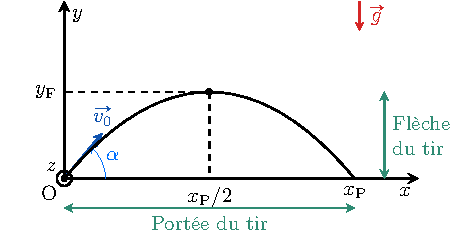
\includegraphics[width=.7\linewidth, draft=true]{cl_ssf-traj}
	}{
		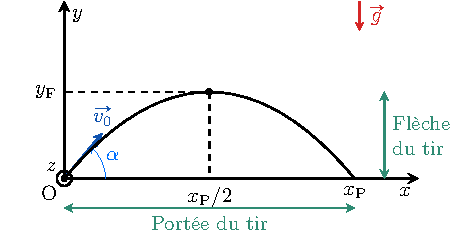
\includegraphics[width=.7\linewidth]{cl_ssf-traj}
	}
	\caption{Chute libre (sans frottements).}
	\label{fig:cl_ssf-traj}
\end{figure}

On peut en définir deux caractéristiques principales, la \textbf{portée} et la
\textbf{flèche}.

\begin{tcb*}(defi){Portée d'un tir}
	\psw{
		La \textbf{portée} d'un tir est la distance \textbf{horizontale} entre
		l'origine du tir et l'endroit où retombe le tir.
	}
\end{tcb*}

Autrement dit, on trouve $x_P$ tel que~:
\psw{
	\begin{gather*}
		y(x_P) = 0
		\\
		\Lra
		x_P\left(- \frac{g}{2v_0{}^2\cos^2\alpha}x_P + \tan\alpha\right) = 0
	\end{gather*}
}
On cherche $x_P \neq 0$ (origine du tir), d'où
\psw{
	\begin{gather*}
		- \frac{g}{2v_0{}^2\cos^2\alpha}x_P + \tan\alpha = 0
		\\
		\Lra
		x_P = \frac{2v_0{}^2\cos^2\alpha}{g}\tan\alpha =
		\frac{2v_0{}^2\cos^{\cancel{2}}\alpha}{g}
		\frac{\sin\alpha}{\cancel{\cos\alpha}}
		\\
		\Lra
		\boxed{x_P = \frac{v_0{}^2}{g}\times 2\sin\alpha\cos\a =
		\frac{v_0{}^2}{g}\sin(2\a)}
	\end{gather*}
}
\vspace{-15pt}

\begin{tcb}[cnt](impl){Portée maximale altitude nulle}
	\psw{
		Ainsi, \xul{pour un tir à altitude nulle}, la portée est maximale si
		$\sin(2\a) = 1$, soit \fbox{$\a = \pi/4$}.
	}
\end{tcb}

\begin{tcb*}(defi){Flèche d'un tir}
	\psw{
		La \textbf{flèche} d'un tir est la \textbf{hauteur maximale} atteinte par le
		projectile.
	}
\end{tcb*}

On trouve $y_F$ quand la vitesse \textbf{verticale} s'annule, $\dot{y}(t_F) = 0$~;
ainsi
\psw{
	\begin{gather*}
		-gt_F + v_0\sin\alpha=0
		\Lra
		t_F = \frac{v_0\sin\a}{g}\\
		\Ra
		y_F = y(t_F) = -\frac{1}{2}g \left( \frac{v_0\sin\a}{g} \right)^2 +
		v_0\sin\a\times \frac{v_0\sin\a}{g}
		\\
		\Lra
		\boxed{y_F = \frac{v_0{}^2}{2g}\sin^2\alpha}
	\end{gather*}
}
\vspace{-15pt}

\begin{tcb}(impl){Flèche maximale}
	\begin{center}
		\psw{
			Le maximum se trouve en $\alpha = \pi/2$.
		}
	\end{center}
\end{tcb}

\begin{tcb*}(appl)<lfnt>'l'{Temps de vol}
	Pour quel angle le temps de vol est-il le plus grand~?
	\tcblower
	\psw{
	Le temps de vol correspond au temps pour lequel le projectile retombe au
	sol, c'est-à-dire $t(x_P)$.
	\smallbreak
	\[
		%\DS
		t_{\max} = t(x_P)
		\Lra
		t_{\max} = \frac{\frac{v_0{}^{\cancel{2}}}{g}\times
		2\sin\a\bcancel{\cos\a}}{\cancel{v_0}\bcancel{\cos\a}}
		\Lra
		\boxed{t_{\max} = 2 \frac{v_0}{g}\sin\a}
	\]
	Le temps de vol est donc maximal pour \fbox{$\alpha = \pi/2$}.
	}
\end{tcb*}

\subsection{Poussée d'\textsc{Archimède}}
\begin{tcb*}(defi){Poussée d'\textsc{Archimède}}
	Lorsqu'un objet est dans un fluide, il subit une force nommée
	\textbf{Poussée d'\textsc{Archimède}} et égale à l'opposé du poids du fluide
	déplacé. Elle est parfois notée $\Pif$ ou $\Ff_A$, et on a~:
	\psw{
		\[\boxed{\Ff_A = -\rho\ind{fluide}V\ind{immergé}\gf}\]
	}
	avec $\rho\ind{fluide}$ la masse volumique du fluide et $V\ind{immergé}$ le
	volume de l'objet qui est dans le fluide.
\end{tcb*}

\begin{tcb*}[breakable](appl)<lfnt>'l'{Glaçon immergé}
	Quelle est la proportion immergée d'un glaçon~? On donne $\rho\ind{eau} =
		\SI{1.00e3}{kg.m^{-3}}$ et $\rho\ind{glace} = \SI{9.17e2}{kg.m^{-3}}$.
	% \vspace{-15pt}
	\tcblower
	%\cswitch{white}{
	\begin{minipage}[t]{0.75\linewidth}
		\psw{
			On suppose un glaçon immobile, donc d'accélération nulle. Il subit son
			poids et la poussée d'\textsc{Archimède}~:
			\begin{gather*}
				\of = \Ff_A + \Pf\\
				\beforetext{Or}
				\Pf = m\gf = \rho\ind{glace}V\ind{glaçon}\gf
				\qet
				\Ff_A = -\rho\ind{eau}V\ind{immergé}\gf
			\end{gather*}
		}
	\end{minipage}
	\hfill
	\begin{minipage}[t]{0.18\linewidth}
		\vspace{-10pt}
		\begin{center}
			\sswitch{
				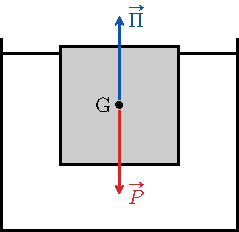
\includegraphics[width=\linewidth, draft=true]{glacon}
			}{
				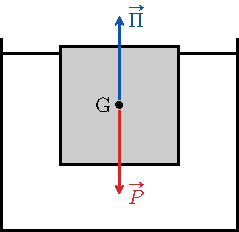
\includegraphics[width=\linewidth]{glacon}
			}
			\vspace{-15pt}
			\captionof{figure}{}
		\end{center}
	\end{minipage}

	\psw{
		D'où
		\begin{gather*}
			-\rho\ind{eau}V\ind{immergé}\cancel{\gf} +
			\rho\ind{glace}V\ind{glaçon}\cancel{\gf}
			\\\Lra
			\boxed{\frac{V\ind{immergé}}{V\ind{glaçon}} =
				\frac{\rho\ind{glace}}{\rho\ind{eau}} = \SI{91.7}{\%}}
		\end{gather*}
		On observe également qu'un objet \textbf{plus dense} que le fluide aura
		une proportion immergée $> 1$~: il ne sera donc pas à l'équilibre
		mécanique et coulera.
	}
\end{tcb*}

\subsection{Frottements fluides}
\subsubsection{Force de frottement fluide}
\begin{tcb*}(defi){Définition}
	Un objet en mouvement dans un fluide subit une force de frottements dite
	fluide $\Ff_f$ qui est une force de \textbf{freinage}, donc \textbf{opposée à
		la vitesse} $\vf$. Selon la norme de la vitesse, on a~:
	\smallbreak
	\begin{isd}
		\tcbsubtitle{\fatbox{Faibles vitesses}}
		\begin{gather*}
			\beforetext{$\Ff_f \propto v$~:}
			\psw{
				\boxed{\Ff_f = -\a\vf}
			}
		\end{gather*}
		%avec $\a$ en \si{kg.s^{-1}}.
		\tcblower
		\tcbsubtitle{\fatbox{Vitesses élevées\ftn{On dit que $\Ff_f$ est
					\textbf{quadratique} selon $v$}}}
		\begin{gather*}
			\beforetext{$\Ff_f \propto v^{2}$~:}
			\psw{
				\boxed{\Ff_f = -\beta v\vf}
			}
		\end{gather*}
		%avec $\beta$ en \si{kg.m^{-1}}.
	\end{isd}
\end{tcb*}

\begin{tcb*}(rema)<lfnt>'l'{Coefficient frottements fluides}
	En pratique, on verra souvent
	\[\beta = \frac{1}{2}\rho\ind{fluide}Sc_x\]
	\begin{itemize}
		\item $\rho\ind{fluide}$ la masse volumique du fluide~;
		\item $S$ la surface
		      frontale («~l'ombre~» que fait l'objet sur un flux)~;
		\item $c_x$ un coefficient
		      sans dimension dépendant surtout de la forme de l'objet.
	\end{itemize}
\end{tcb*}

\subsubsection{Chute libre sans vitesse initiale avec frottements linéaires}
\hspace*{-0.75cm}
\begin{minipage}[t]{0.65\linewidth}
	\begin{enumerate}[label=\sqenumi]
		\bitem{Système.} \{bille\} dans une
		éprouvette d'huile dans $\Rc\ind{labo}$, supposé galiléen.
		\bitem{Schéma.}
	\end{enumerate}
\end{minipage}
\hfill
\begin{minipage}[t]{0.30\linewidth}
	\begin{center}
		\vspace{-12pt}
		\sswitch{
			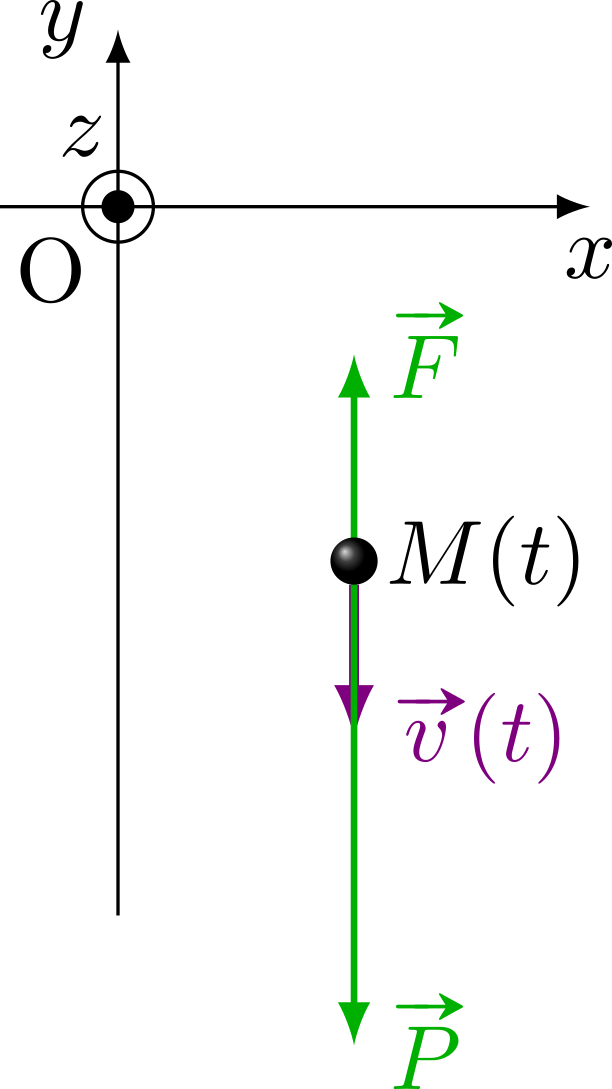
\includegraphics[height=4cm, draft=true]{cl_fl}
		}{
			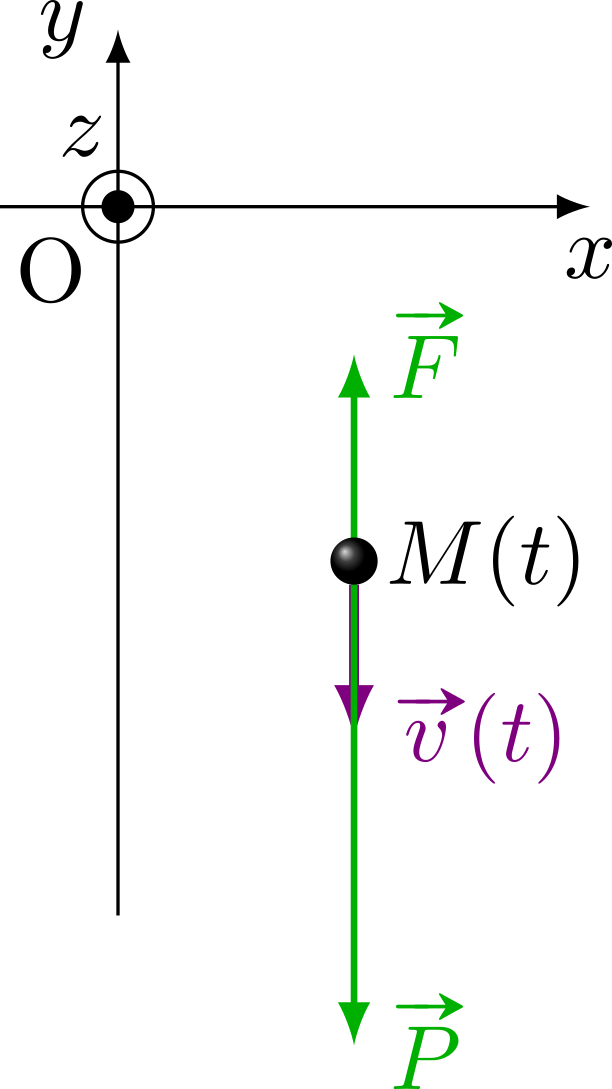
\includegraphics[height=4cm]{cl_fl}
		}
		\captionof{figure}{Schéma.}
	\end{center}
\end{minipage}
\vspace{-55pt}
\begin{enumerate}[label=\sqenumi, start=3]
	\bitem{Modélisation.}
	\begin{itemize}
		\item Repère~: $(\ux,\uy,\uz)$ BOND avec $\uy$ verticale ascendante.
		\item Repérage~:
		      \psw{
			      \begin{align*}
				      \OM & = y\uy    \\
				      \vf & = \yp\uy  \\
				      \af & = \ypp\uy
			      \end{align*}
		      }
		      \vspace{-15pt}
		\item Conditions initiales~: $\OM(0)$ position de la bille lors de son
		      entrée dans le glycérol~; $\vf(0) = \of$.
		\item On néglige pour simplifier la poussée d’\textbf{Archimède}.
	\end{itemize}
	\bitem{Bilan des forces.}
	\psw{
		\[
			\begin{array}{ll}
				\textbf{Poids}              & \Pf = m\gf = -mg\uy            \\
				\textbf{Frottements fluide} & \Ff_f = -\a\vf = -\a\dot{y}\uy
			\end{array}
		\]
	}
	\item \leftcenters{\textbf{PFD.}}{\psw{$m\af = \Pf + \Ff$}}
	      \bitem{Équations scalaires}.
	      \psw{
		      \[
			      m \dv{\yp}{t} = -mg -\alpha \yp
		      \]
	      }
	      \vspace{-15pt}
	      \bitem{Répondre aux questions.} On obtient ici trois équations
	      différentielles sur la vitesse ($v_x = \xp$, $v_y = \yp$ et $v_z =
		      \zp$), mais en absence de vitesse initiale sur $v_x$ et $v_z$, il n'y
	      aura pas de mouvement sur ces coordonnées~: on s'intéresse donc à
	      l'équation différentielle sur $v_y$ que l'on appelle simplement $v$,
	      avec $\tau = m/\a$~:
	      \psw{
		      \[
			      \boxed{\dv{v}{t} + \frac{\alpha}{m}v = -g}
			      \Lra
			      \dv{v}{t} + \frac{v}{\tau} = -g
		      \]
	      }
\end{enumerate}

Une résolution complète demande de discerner solution homogène et particulière
puis d'utiliser les conditions initiales, pour trouver
\[v(t) = g\tau\left(\exr^{-t/\tau}-1\right)\]

On peut développer une autre approche générique pour obtenir des grandeurs
typiques d'un système à partir de l'équation différentielle qui régit son
fonctionnement~: l'\textbf{adimensionnement}. \bigbreak

On définit $v^* = v/V$, $t^* = t/T$ avec $V$ et $T$ des constantes à définir. On
peut donc réécrire
\psw{
	\begin{gather*}
		\frac{V}{T} \dv{v^*}{t^*} + \frac{\a}{m}Vv^* = -g
		\\\Lra
		\dv{v^*}{t^*} + \frac{\a T}{m}v^* = - \frac{gT}{V}
	\end{gather*}
}
On choisit alors $T$ et $V$ de façon à écrire
\begin{gather*}
	\psw{\boxed{\dv{v^*}{t^*} + v^* = -1}}
	\qav
	\psw{\boxed{T = \frac{m}{\a}}}
	\qet
	\psw{\boxed{V = gT = \frac{gm}{\a}}}
\end{gather*}

Dans ces conditions, l'équation différentielle adimensionnée donne $T$
\textbf{grandeur typique du temps} d'évolution de la vitesse, et $V$ est la
\textbf{vitesse atteinte en régime permanent}.

\begin{figure}[htbp!]
	\centering
	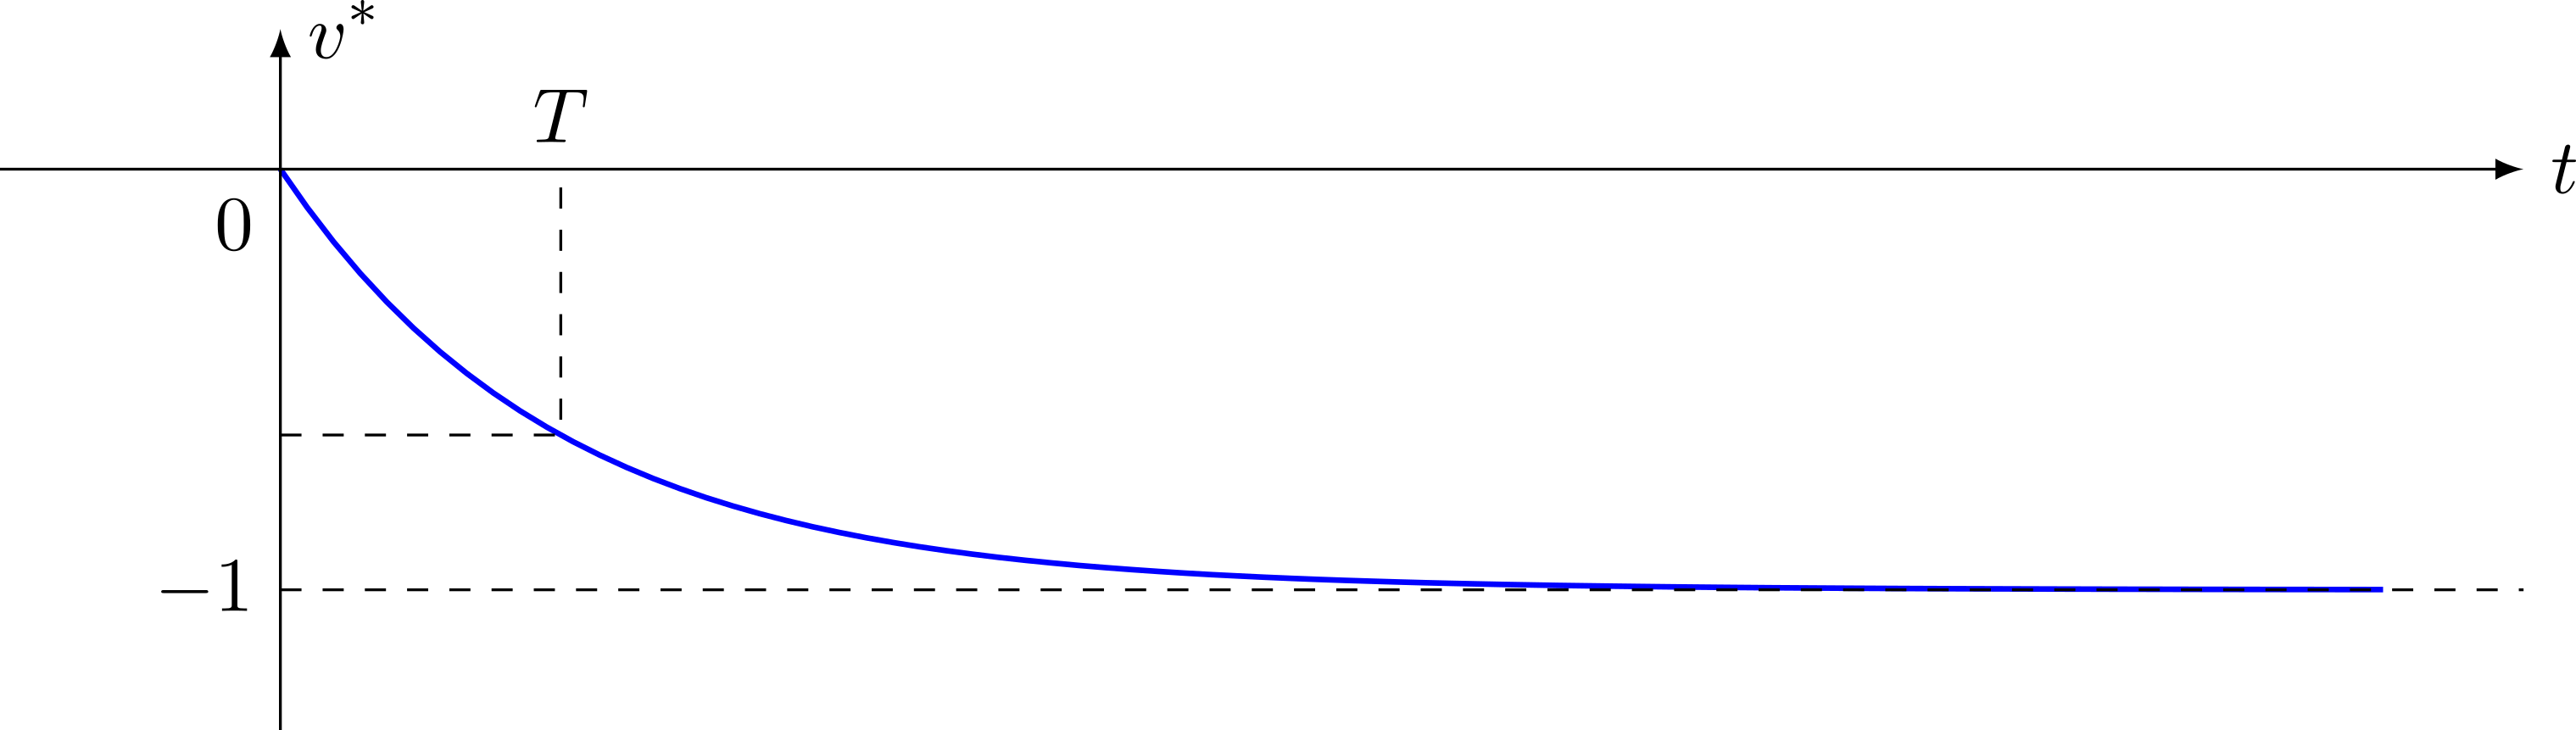
\includegraphics[width=.7\linewidth]{cl_fl-v}
	\caption{Évolution de $v^{*}$ avec le temps}
	\label{fig:cl_fl-v}
\end{figure}

\begin{tcb*}(defi){Équations adimensionnées}
	L'écriture sous forme adimensionnée permet de ramener la résolution de
	l'équation à un problème uniquement mathématique, débarrassé des constantes
	physiques et permettant de voir rapidement le fonctionnement d'un système même
	quand on ne sait pas résoudre l'équation.
\end{tcb*}

\subsubsection{Chute libre sans vitesse initiale avec frottements quadratiques}

Pour une chute libre dans l'air, la vitesse d'un corps est presque toujours
suffisamment élevée pour que les frottements soient quadratiques en la vitesse.
On choisit ici $\uy$ vers le bas, tel que $v = \yp > 0$. Ainsi, une chute
totalement verticale donne
\psw{
	\[\Ff_f = -\beta\yp^2\uy\]
}
Toujours en négligeant la poussée d'\textsc{Archimède}, on a
\psw{
	\[\dv{v}{t} + \frac{\beta}{m}v^2 = g\]
}
La résolutions analytique exacte de cette équation sort du cadre du programme~;
on peut en revanche \textbf{l'adimensionner pour trouver ses grandeurs typiques}.
On définit $v^* = v/V$, $t^* = t/T$ avec $V$ et $T$ des constantes à définir. On
peut donc réécrire
\psw{
	\begin{gather*}
		\frac{V}{T} \dv{v^*}{t^*} + \frac{\beta}{m}V^2(v^*)^2 = g
		\\\Lra
		\dv{v^*}{t^*} + \frac{\beta}{m}VT(v^*)^2 = \frac{gT}{V}
	\end{gather*}
}
On choisit alors $T$ et $V$ de façon à écrire
\begin{gather*}
	\psw{\boxed{\dv{v^*}{t^*} + (v^*)^2 = 1}}
	\qav
	\psw{\boxed{T = \sqrt{\frac{m}{\beta g}}}}
	\qet
	\psw{\boxed{V = gT = \sqrt{\frac{mg}{\beta}}}}
\end{gather*}

Dans ces conditions, l'équation différentielle adimensionnée donne $T$ grandeur
typique du temps d'évolution de la vitesse, et $V$ est la vitesse atteinte en
régime permanent.

Avec pour un-e humain-e en chute libre sans parachute, on a
$\beta \approx \SI{0.25}{kg.m^{-1}}$, soit
\psw{
	\[
		\boxed{v_{\lim} = \SI{60}{m.s^{-1} \approx \SI{200}{km.h^{-1}}}}
		\qet
		\boxed{T \approx \SI{6}{s}}
	\]
}

% TODO: schéma solution frottements quadratiques python

\subsection{Force de frottements solides}
\subsubsection{Réaction d'un support}

\begin{tcb*}[sidebyside, righthand ratio=.4](defi){Réaction d'un support}
	La force exercée par un support sur un objet posé à sa surface est appelée
	\textbf{réaction} et est notée $\Rf$. Elle se décompose en deux forces~:
	\psw{
		\[
			\Rf = \Nf + \Tf
			\qou
			\Rf = \Rf_N + \Rf_T
		\]
	}
	\vspace{-15pt}
	\begin{itemize}
		\item $\Nf$ \psw{\textbf{normale} ($\perp$) au support~;}
		\item $\Tf$ \psw{
			      \textbf{tangentielle} ($\parr$) au support, \textbf{opposée} à la
			      vitesse. }
	\end{itemize}
	\tcblower
	\begin{center}
		\sswitch{
			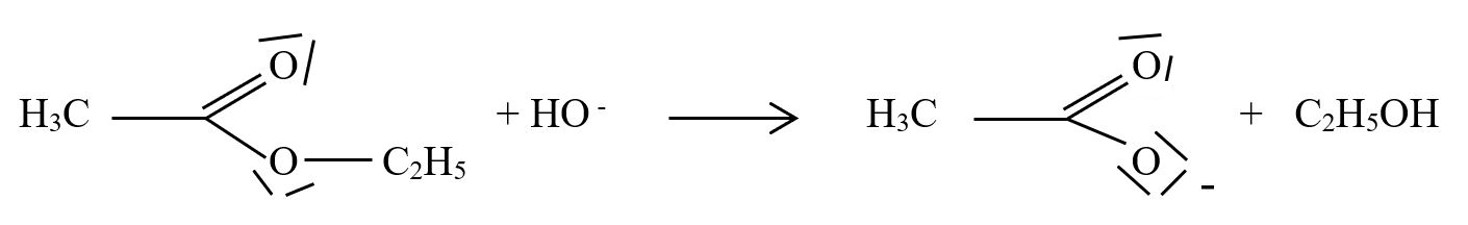
\includegraphics[width=\linewidth, draft=true]{reaction}
		}{
			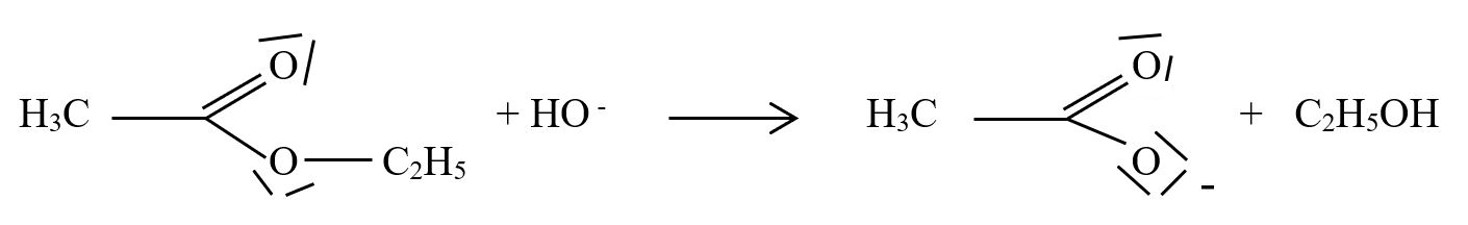
\includegraphics[width=\linewidth]{reaction}
		}
		\vspace{-15pt}
		\captionof{figure}{Réaction du support}
	\end{center}
\end{tcb*}
\begin{tcb*}[cnt, bld](ror){Condition de support}
	\psw{La \textbf{condition de support} est $\norm{\Nf} > 0$.}
\end{tcb*}

\subsubsection{Lois de \textsc{Coulomb}}
Les relations entre les \textbf{normes} des forces $\Nf$ et $\Tf$ sont appelées
\textbf{lois du frottement de \textsc{Coulomb}}.

\begin{tcb*}(prop){Lois du frottement de \textsc{Coulomb}}
	Les réactions normales et tangentielles sont reliées par les lois de
	\textsc{Coulomb}, telles que~:
	\smallbreak
	\begin{isd}
		\tcbsubtitle{\fatbox{Solide glissant}}
		\psw{
			\[
				\norm{\Tf} = f\norm{\Nf}
				\qou
				\norm{\Tf} = f_d \norm{\Nf}
			\]
		}
		\tcblower
		\tcbsubtitle{\fatbox{Solide non-glissant}}
		\psw{
			\[
				\norm{\Tf} < f\norm{\Nf}
				\qou
				\norm{\Tf} = f_s \norm{\Nf}
			\]
		}
	\end{isd}
	% avec $f_s$ le coefficient de frottement solides \textbf{dynamique} et $f_s$
	% le \textbf{statique}. Ce sont des nombres sans
	$f$ le coefficient de frottements solides. C'est un nombre sans
	dimension, souvent inférieur à 1 et qui dépend de l'\textbf{état} de la
	surface (humide, graissée) mais \textbf{pas de son aire}.
	\bigbreak
	De manière plus particulière, on définit $f_d$ le coefficient de frottements
	dynamiques (glissement) et $f_s$ le coefficient de frottement statique (pas
	glissement), avec $f_d < f_s$~; dans ce cas, $f = f_d$.
	% On définit généralement \textbf{un seul} coefficient de frottements solides,
	% $\boxed{f_d = f}$.
\end{tcb*}

\begin{tcb*}(impo)<lfnt>'l'{Absence de frottements solides}
	L'absence de frottements solides implique $f=0$, donc $T = 0$, mais
	\textbf{la force normale n'est jamais nulle}.
\end{tcb*}

\subsection{Force de rappel d'un ressort}
\subsubsection{Force de rappel élastique}

\begin{tcb*}[sidebyside, righthand ratio=.45](defi){Force de rappel d'un ressort}

	Soit le système masse-ressort horizontal représenté ci-contre. Le ressort se
	déforme sous l'effet d'une contrainte en stockant l'énergie donnée, qu'il
	libère en reprenant sa forme quand la contrainte s'arrête. On définit la
	force de rappel du ressort par~:
	\begin{equation*}
		\psw{\boxed{\vv*{F}{\rm rappel} = \pm k(\ell - \ell_0)\ur}}
	\end{equation*}
	\begin{itemize}
		\item $k > 0$ la \textbf{constante de raideur}~;
		\item $\ell_0$ sa \textbf{longueur à vide}~;
		\item $\ur$ unitaire dirigé selon l'axe du ressort.
	\end{itemize}
	\begin{center}
		Elle est aussi appelée \textbf{force de \textsc{Hooke}}.
	\end{center}
	\tcblower
	\begin{center}
		\sswitch{
			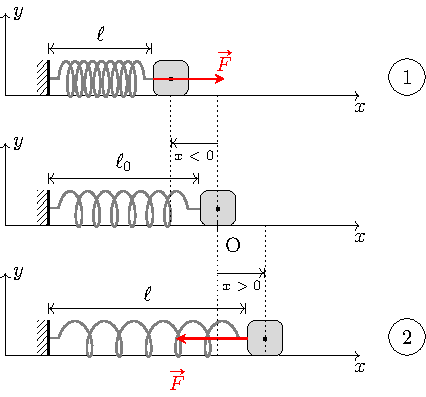
\includegraphics[width=\linewidth, draft=true]{ressort_def}
		}{
			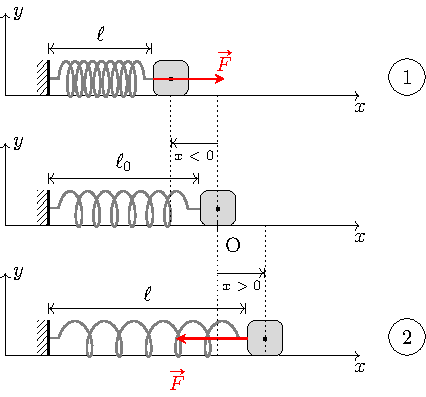
\includegraphics[width=\linewidth]{ressort_def}
		}
		\vspace{-15pt}
		\captionof{figure}{Force de \textsc{Hooke}.}
	\end{center}
	% Si $\ell > \ell_0$, on a bien une force dirigée selon $-\ux$, (situation
	% \circled{2}), sinon dirigée selon $+\ux$.
\end{tcb*}

\begin{tcb*}(impo){Signe $\pm$}
	Le signe de la force dépend du repère~: de façon générale, il faut
	regarder le sens dans lequel s’exerce la force si on étire le ressort ($(\ell
		- \ell_0) > 0$) et placer le signe en conséquence.
\end{tcb*}

\subsubsection{Position d'équilibre verticale}
\vspace*{-.7cm}
\noindent
\begin{minipage}{0.75\linewidth}
	À l'horizontale, on voit vite que $\ell\ind{eq} = \ell_0$. À la verticale,
	$\ell\ind{eq} > \ell_0$ à cause du poids. Quelle est son expression~?
	\begin{enumerate}[label=\sqenumi]
		\bitem{Système}~: \{masse\} accrochée à un ressort, représenté par M de masse
		$m$.
		\bitem{Référentiel}~: $\Rc(O,\ux,\uz)$ galiléen.
		\bitem{Repère}~: $(\Or, \uz)$ vertical ascendant.
	\end{enumerate}
\end{minipage}
\hfill
\begin{minipage}{.25\linewidth}
	\begin{center}
		\sswitch{
			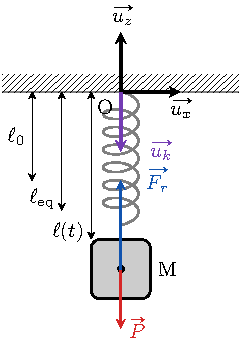
\includegraphics[width=.7\linewidth, draft=true]{ressort_vert}
		}{
			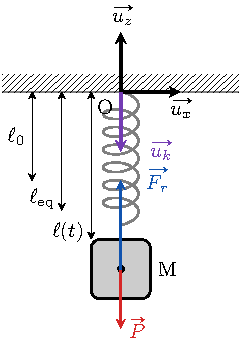
\includegraphics[width=.7\linewidth]{ressort_vert}
		}
		\captionof{figure}{}
	\end{center}
\end{minipage}

\vspace{-20pt}
\begin{enumerate}[label=\sqenumi, start=4]
	\bitem{BdF}~:
	\psw{
		\[
			\begin{array}{ll}
				\textbf{Poids}                & \Pf = m\gf = -mg\uz       \\
				\textbf{Force \textsc{Hooke}} & \Ff = k(\ell - \ell_0)\uz
			\end{array}
		\]
	}
	\bitem{PFD à l'équilibre}~:
	\vspace{-22pt}
	\psw{
		\begin{gather*}
			0 = -mg + k(\ell_{\equ} - \ell_0)
			\Lra
			k(\ell_{\equ} - \ell_0) = mg
			\\\Lra
			\boxed{\ell_{\equ} = \ell_0 + \frac{mg}{k}}
		\end{gather*}
	}
	D'où
	\[
		\psw{m \text{ ou } g \nearrow \Ra \ell\ind{eq} \nearrow}
		\qet
		\psw{k \nearrow \Ra \ell\ind{eq} \searrow}
	\]
\end{enumerate}
\vspace{-15pt}

\end{document}
